\part{Telemetry System Design}

The telemetry system being designed for the 2025 launches is designed to be flown in both competition rockets: the
30,000ft \gls{cots} solid motor at \gls{sac} and the hybrid motor rocket at \gls{lc}.

This year's telemetry system aims to address the shortcomings in last year's design. The main flaws that are being
addressed are:

\begin{itemize}
    \item Battery life status updates
    \item Power consumption
    \item System size for physical placement in the rocket
    \item Radio signal strength
    \item Enclosure integrity under shock load
    \item Lack of sensor fusion and equal data acquisition
    \item Use of memory for data logging while the rocket is idle
\end{itemize}

\section{Hardware Design}

The telemetry system is composed of two \gls{srad} \gls{pcb}s. One \gls{mcu} \gls{pcb} which as well as containing the
\gls{mcu} also includes all the sensors and power circuitry essential to making the telemetry system work. The other
\gls{srad} \gls{pcb} is the radio board responsible for transmitting information from the rocket to the ground station
which is the same \gls{pcb} as the radio board with different features utilized. All of these subsystems are explored
in more depth in the following sections.

\subsection{Microcontroller Unit Selection}

The microcontroller unit selected for the telemetry system flight computer is an STM32H743VI. Key specifications are as
follows:

\begin{itemize}
    \item Single ARM Cortex M7 up to 480MHz \cite[1]{stm32h743vi}
    \item 32KB split L1 cache \cite[1]{stm32h743vi}
    \item 2MB flash memory \cite[1]{stm32h743vi}
    \item 1MB SRAM \cite[1]{stm32h743vi}
    \item DFU programming \cite[Sec. 3.4]{stm32h743vi}
    \item Multiple power domains \cite[1]{stm32h743vi}
    \item 2.43uA in standby mode \cite[1]{stm32h743vi}
    \item 275uA/MHz at 3.3V in run mode \cite[1]{stm32h743vi}
    \item Double precision \gls{fpu} \cite[1]{stm32h743vi}
\end{itemize}

\Gls{cuinspace} will be under-clocking the \gls{mcu} to around \qty{250}{\mega\hertz} to further reduce power consumption, as this frequency should be sufficient for our application.

The STM32H743 was selected for its power efficiency, large number of peripherals and NuttX support. It's single-core
architecture makes it simple to program, as many of the other \glspl{mcu} in the STM32H7 series have a dual asymmetric
core architecture. Its DFU bootloader will be leveraged to program the chip over USB, which is a more common interface
available to \gls{cuinspace} members than ST-Link/JTAG programmers.

The \gls{io} from this \gls{mcu} used in this system are summarized in \Cref{tab:mcu-io}. This is also shown in
graphical representation in \Cref{fig:mcu-diagram}. The primary reasons for selecting this \gls{mcu} were:

\begin{itemize}
    \item Low power consumption
    \item Ample processing power, \gls{sram}, and flash memory
    \item Excellent power efficiency
    \item Many \gls{io} options
    \item NuttX support
    \item Ease of development
    \item Floating point unit
\end{itemize}

\begin{figure}[H]
    \centering
    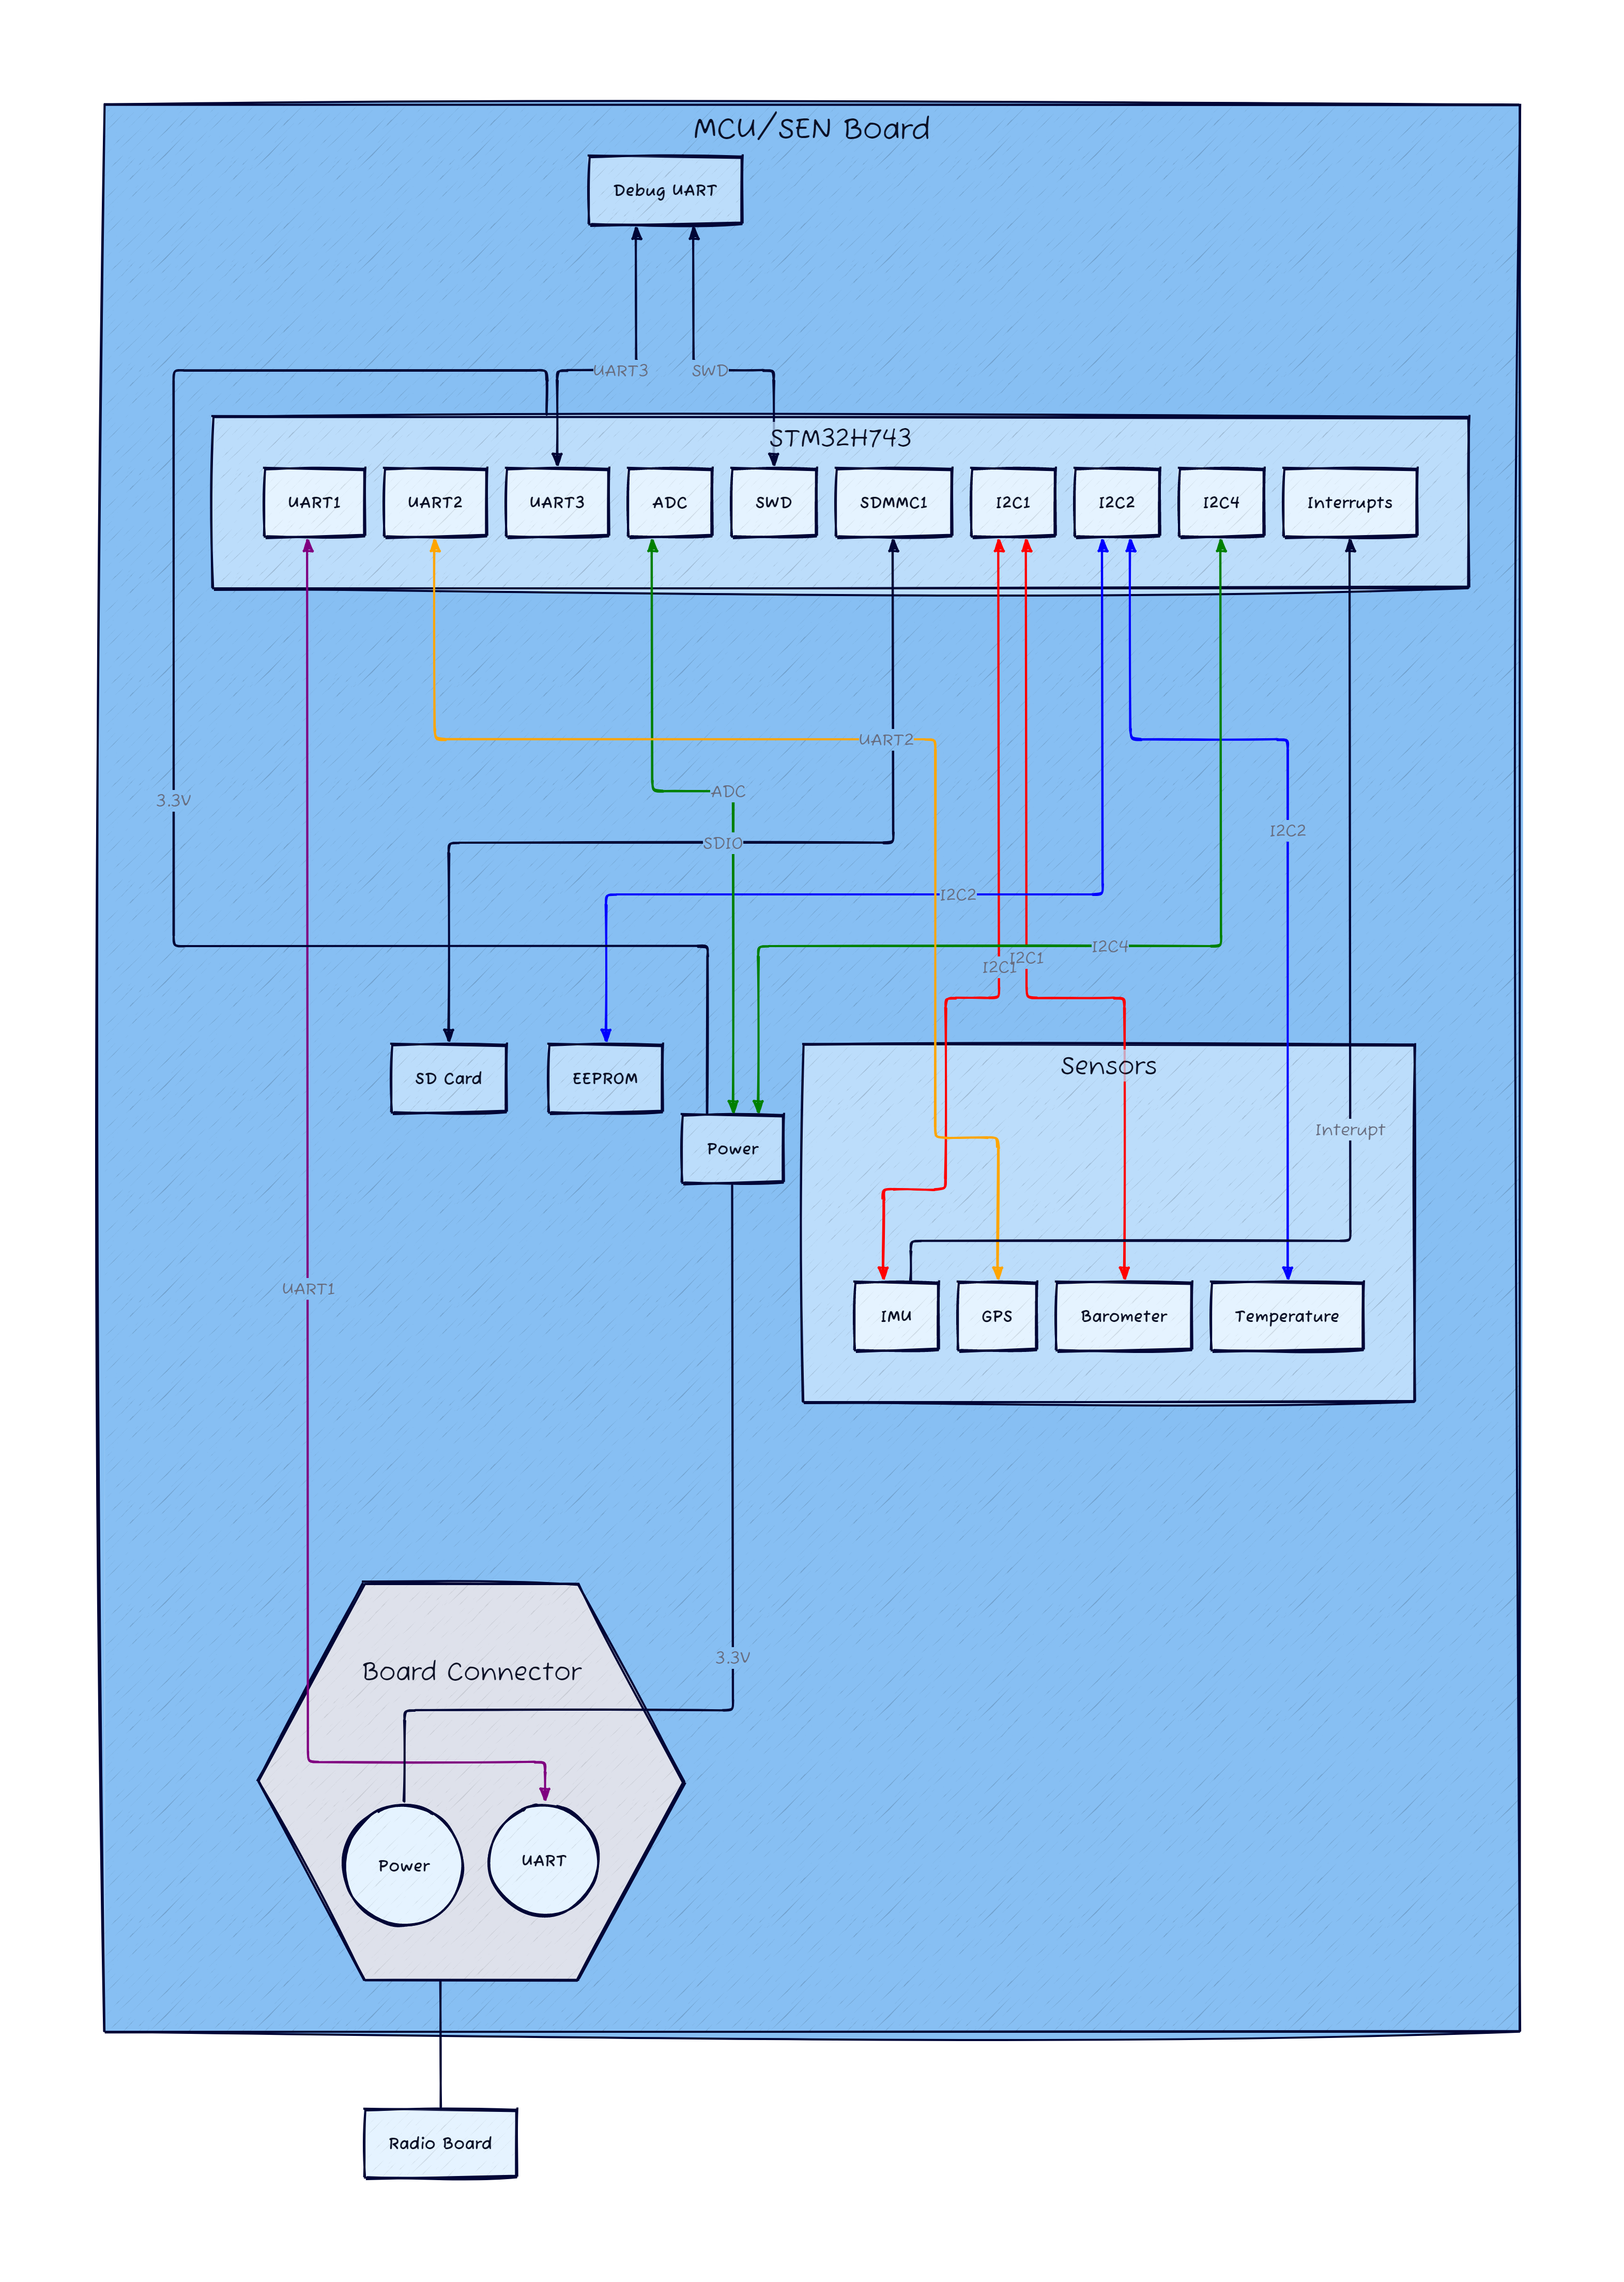
\includegraphics[width=0.8\textwidth]{assets/diagrams/mcu_board.png}
    \caption{STM32H743 \gls{mcu} \gls{io} diagram}
    \label{fig:mcu-diagram}
\end{figure}

\begin{table}[H]
    \centering
    \begin{tabular}{cc}
        \toprule
        \textbf{\gls{io} Bus} & \textbf{Used For}                                          \\
        \midrule
        I2C1                  & \gls{imu} \& Barometer                                     \\
        I2C2                  & \gls{eeprom} \& Temperature \textbackslash Humidity Sensor \\
        I2C4                  & Current Sensor                                             \\
        UART1                 & Radio                                                      \\
        UART2                 & \gls{gps}                                                  \\
        UART3                 & Debug                                                      \\
        SDMMC1                & MicroSD Card                                               \\
        SWD                   & Debug                                                      \\
        \gls{adc}             & Battery Voltage Detection                                  \\
        \gls{usb}             & Programming \& Debug                                       \\
        \bottomrule
    \end{tabular}
    \caption{\gls{mcu} \gls{io} usage}
    \label{tab:mcu-io}
\end{table}

\subsection{Power System}

\begin{figure}[H]
    \centering
    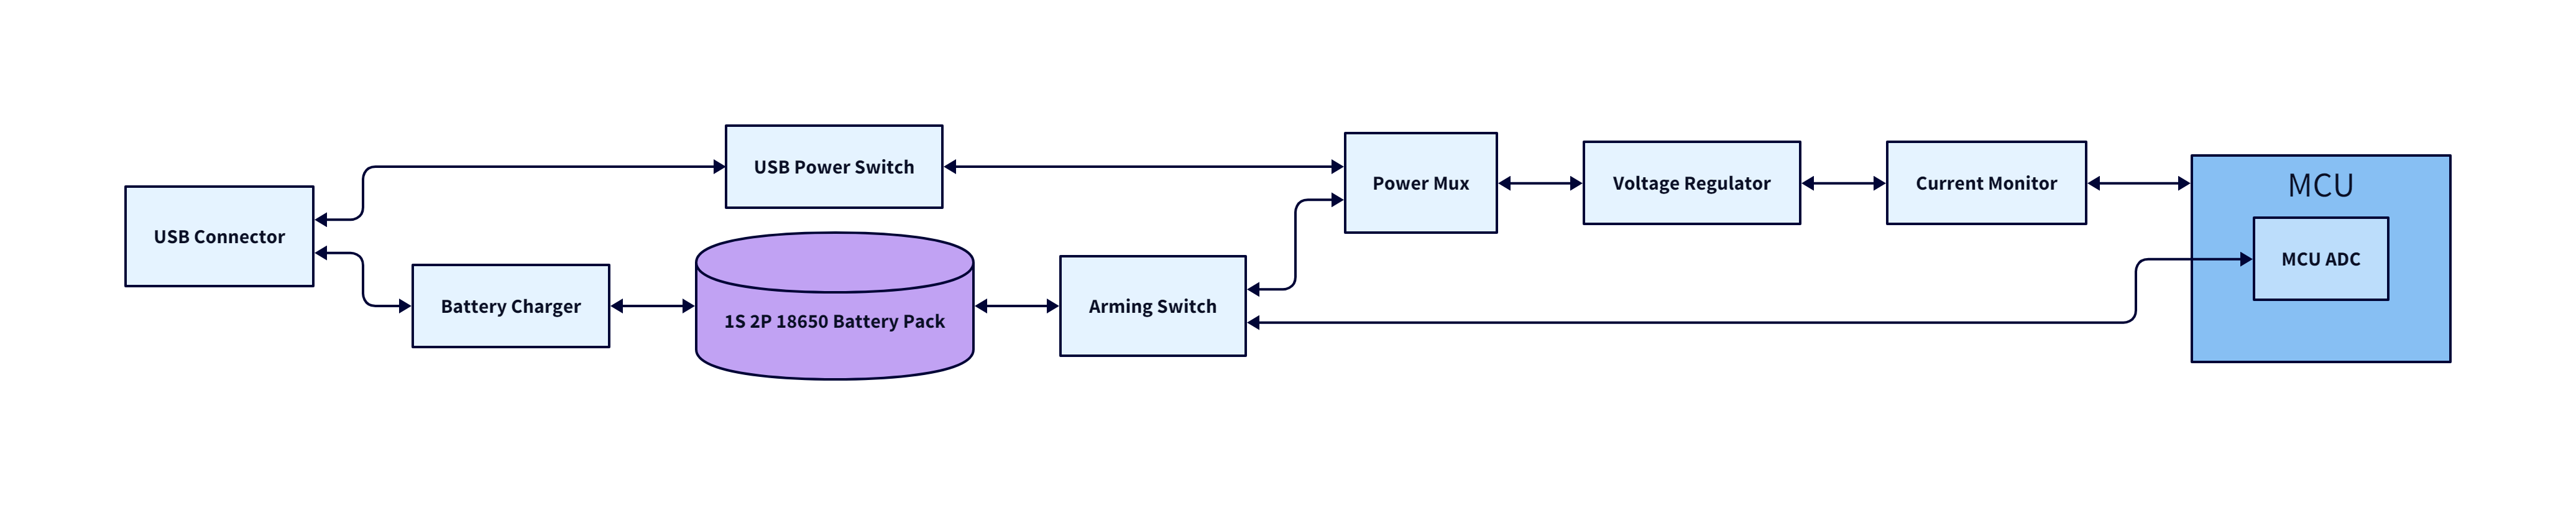
\includegraphics[width=\linewidth]{assets/diagrams/power_system.png}
    \caption{Power system architecture}
    \label{fig:power-system}
\end{figure}

The selected nominal supply voltage for all components in the telemetry system is 3.3V. This voltage is used for both
the \gls{mcu} board and the radio transmitter board, which will be supplied from the \gls{mcu} board.

The current draw budgeting for all the components in the telemetry system can be seen in \Cref{tbl:draw}.

\begin{table}[H]
    \centering
    \caption{Current draw breakdown for each component in the telemetry system}
    \label{tbl:draw}
    \begin{tabular}{p{0.8in} p{0.5in} p{0.5in} p{0.5in} p{0.5in} p{0.5in} p{0.5in}}
        \hline
        MS5607      & 1.25 & 0.0002 & 10  & 90 & 0.125 & 1.25  \\
        \hline
        SHT41       & 0.5  & 0.05   & 10  & 90 & 0.095 & 1     \\
        \hline
        L86-M33 GPS & 36.0 & 1      & 100 & 0  & 36.0  & 100.0 \\
        \hline
        SD card     & 50.0 & 1.25   & 60  & 40 & 30.5  & 200.0 \\
        \hline
        EEPROM      & 3.0  & 0.001  & 2   & 98 & 0.061 & 3.0   \\
        \hline
        MCU         & 34.0 & -      & 100 & 0  & 24.0  & 100.0 \\
        \bottomrule
    \end{tabular}
\end{table}

\subsubsection{Supplies}

Due to restrictions imposed by \gls{sac} competition regulations, the \gls{cuinspace} telemetry system is designed to
be powered using standard 18650 \glspl{lion} with a \gls{jst} connector. The nominal voltage of these batteries is
3.7V, which is sufficient to meet the selected nominal supply voltage of 3.3V.

For debugging purposes, power can also be supplied over a USB connection at 5V.

\subsubsection{Power Regulation}

To regulate the voltages from both power supplies, \gls{cuinspace} has selected a \gls{ldo} voltage regulator.
\Gls{ldo} regulators have a lower power efficiency when compared with switching voltage regulators, but they have a
much lower noise floor. A switching voltage regulator can operate from a few hundred kilohertz to the megahertz
switching frequency range. Higher frequency noise is easier to filter out for the sensor networks, which are more
susceptible to low frequency noise, but high frequency noise has an adverse effect on radio signals.

To avoid both issues, a \gls{ldo} regulator sacrifices some efficiency in return for less noise.

\subsection{Sensor Systems}

The sensors on board the flight computer are required to collect information about the rocket's state during flight at
a high enough resolution to be able to characterize the rocket's flight path after recovering flight logs or when
receiving telemetry data.

The key pieces of data for a rocket flight are:

\begin{itemize}
    \item Roll, pitch, and yaw
    \item Acceleration in all 3 axes
    \item Velocity in all 3 axes
    \item Altitude
    \item Position
\end{itemize}

With this information it is possible to characterize the rocket's flight path and recover the rocket upon landing. This
information will be logged at a minimum of 10Hz to provide satisfactory resolution of the rocket flight.
\gls{cuinspace} is designing for a minimum of a 10Hz logging rate, but will aim to maximize logging rate on sensors
that are capable of updating faster.

\Gls{cuinspace} also wishes to acquire temperature and humidity information at a lower priority to determine the temperature levels inside the rocket. Since \gls{sac} typically takes place in the New Mexico desert during summer, it is important to characterize temperatures inside the rocket when evaluating thermals on components with important thermal considerations, such as voltage regulators. \Gls{cuinspace} aims to avoid the possibility of any overheating components, or components operating outside their nominal temperature range.

In order to acquire the key pieces of data mentioned above, the following sensors will be used:

\begin{itemize}
    \item Barometric pressure sensor (altitude)
    \item 3-axis magnetometer (compass heading)
    \item 6-axis \acrfull{imu} (linear acceleration) \& (angular velocity)
    \item Temperature and humidity sensor
    \item GNSS chip (positioning, heading, altitude)
\end{itemize}

Many of these sensors require calibration and selection of specific operating settings. To accommodate this need, an
on-board \gls{eeprom} will be used for storing calibration information. This allows multiple boards to be calibrated
after manufacture so they are ready for flight.

\subsubsection{Barometric Pressure Sensor}

The selected barometric pressure sensor is the MS5607.

\begin{figure}[H]
    \centering
    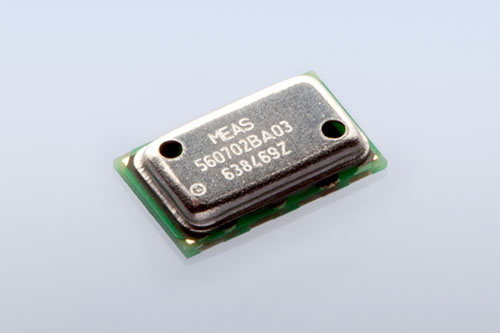
\includegraphics[width=2in]{assets/images/ms5607.jpg}
    \caption{MS5607 barometric pressure sensor \cite{ms5607-pic}}
\end{figure}

The M5607 was selected because it provides an \gls{i2c} interface and operates at a 3.3V supply voltage.
\cite[1]{ms5607-datasheet} It has a resolution of 20 centimetres \cite[1]{ms5607-datasheet} and operates from -40 to 85
degrees Celsius and 10 to 2000 millibars \cite[1]{ms5607-datasheet}, which is well within the expected temperature and
pressure ranges.

\subsubsection{Accelerometer \& Gyroscope}

The selected \gls{imu} is the LSM6DSO32, which combines both 3-axis accelerometer and 3-axis gyroscope in one package.

\begin{figure}[H]
    \centering
    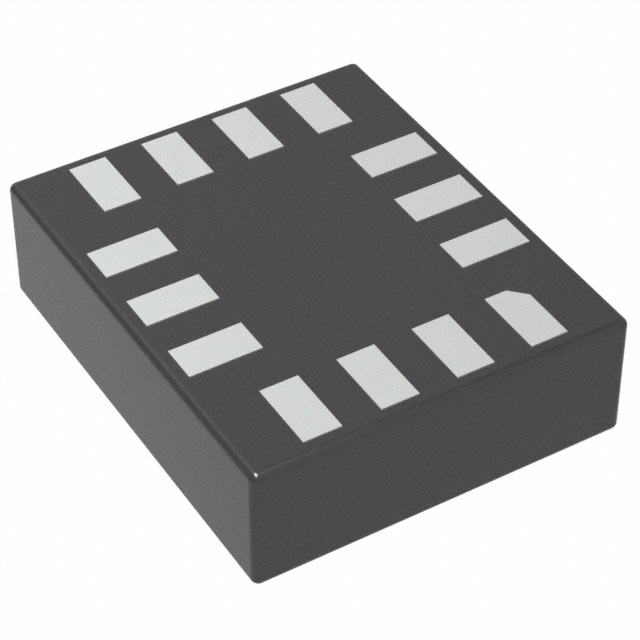
\includegraphics[width=1in]{assets/images/lsm6dso32.jpg}
    \caption{LSM6DSO32 \gls{imu} \cite{lsm6dso32-pic}}
\end{figure}

The LSM6DSO32 was selected because it provides and \gls{i2c} interface and operates at our supply voltage of 3.3V.
\cite{lsm6dso32-datasheet} It also provides a \gls{fsr} of $\pm 32$g \cite[1]{lsm6dso32-datasheet}, which is required
since the rockets flown by \gls{cuinspace} often experience up to around 25g of acceleration at lift-off. This sensor
also has a convenient register interface for reading the sensor and interacting with it.

\subsubsection{Magnetometer}

The selected magnetometer is the LIS2MDL.

\begin{figure}[H]
    \centering
    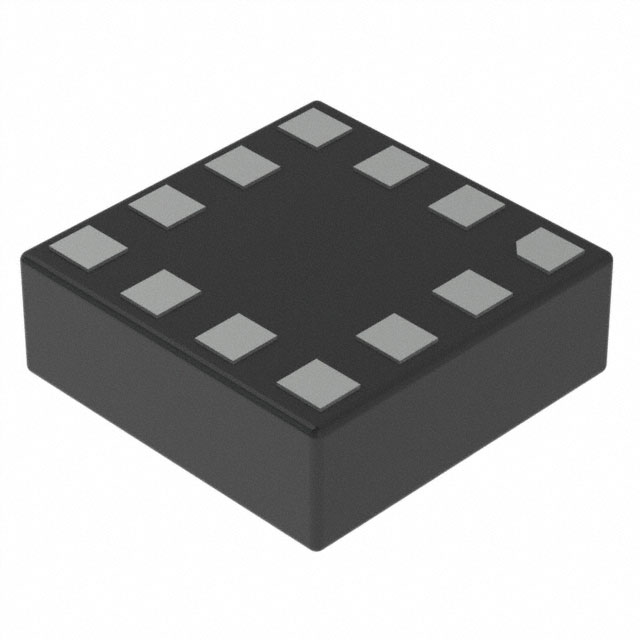
\includegraphics[width=1in]{assets/images/lis2mdl.jpg}
    \caption{LIS2MDL magnetometer \cite{lis2dml-pic}}
    \label{fig:magnetometer}
\end{figure}

This magnetometer was selected because it has an \gls{i2c} interface and can be supplied at 3.3V.
\cite{lis2mdl-datasheet} It also has a convenient register interface similar to the LSM6DSO32, which makes it easy for
\gls{cuinspace} members to user.

\subsubsection{GPS/GNSS}

The selected \gls{gps} and \gls{gnss} receiver module is the Quectel L86-M33.

\begin{figure}[H]
    \center
    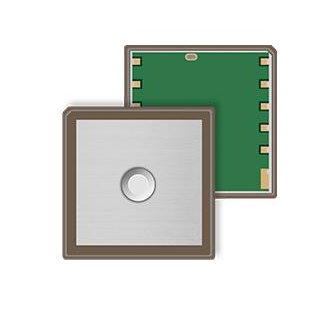
\includegraphics[width=2in]{assets/images/l86m33.png}
    \caption{The L86-M33 \gls{gps} module \cite{gps-pic}}
    \label{fig:gps}
\end{figure}

This \gls{gps} module was selected because it operates at a nominal supply voltage of 3.3V \cite{gps-datasheet} and has
a \gls{uart} interface for sending \gls{nmea} protocol messages. \cite{gps-datasheet} It allows for the use of either
its integrated ceramic antenna or an external antenna \cite{gps-datasheet}. This provides a backup option if the
external antenna design has flaws or if the flight computer is used in an enclosed space where an external \gls{gps}
antenna cannot be used. The module also supports an update frequency of 10 hertz \cite{gps-datasheet}, which meets
\gls{cuinspace}'s minimum requirements. The unit is also around 50\% cheaper than Ublox branded alternatives.

\subsubsection{Temperature \& Humidity Sensor}

The selected temperature and humidity sensor is the Sensirion SHT41.

\begin{figure}[H]
    \centering
    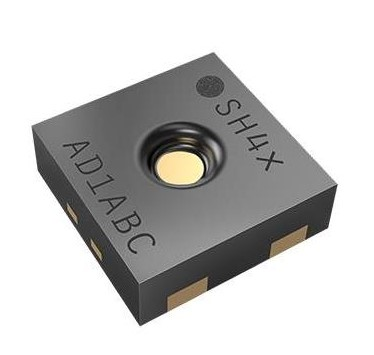
\includegraphics[width=2in]{assets/images/sht41.jpg}
    \caption{The SHT41 temperature and humidity sensor \cite{sht41-pic}}
\end{figure}

This sensor was selected because it has an operating range of -40 to 125 degrees Celsius \cite[1]{sht4x-datasheet},
which covers the operating range of our rocket in both the New Mexico desert and Ontario boreal forests. It can be
supplied at 3.3V \cite[1]{sht4x-datasheet} and is very low power with an average current draw of 0.4 micro-amps.
\cite[1]{sht4x-datasheet} It has an incredibly simple \gls{i2c} control interface which makes it easy to operate.
\cite[Sec. 4.5]{sht4x-datasheet}

\section{Radio Frequency Design}

The radio transmitter portion of the telemetry system will be based on a student-designed \gls{pcb} designed around the
RN2483 radio transceiver chip. More information about the chip's specifications can be found in Appendix
\ref{apx:rn483}. You can see the chip featured on the Pictail board in Figure \ref{fig:pictail}

\begin{figure}[H]
    \centering
    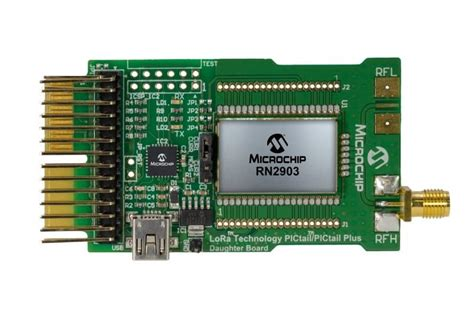
\includegraphics[width=2.5in]{assets/images/pictail.jpg}
    \caption{The RN2483 radio transceiver chip on the commercial Pictail board \cite{pictail-img}}
    \label{fig:pictail}
\end{figure}

The RN2483 chip was selected because of its low power consumption of 38.9 milliamps when transmitting \cite[Table
    2-3]{rn2483-datasheet} and long-range capabilities, transmitting up to a distance of 15 kilometres in suburban
environments \cite[1]{rn2483-datasheet}. It also has a \gls{cots} twin, the RN2483 Pictail board. This is useful to
compare our \gls{srad} designs against during range testing.

\subsection{Radio Parameters}

\subsubsection{Frequency}

The RN2483 transceiver will be used to operate on the 433MHz band in our systems. This frequency band was selected
because it requires a lower transmit power for the same range \cite[Table 2-5]{rn2483-datasheet} as the 868MHz band.
This band is also licensed as a \gls{ham-radio} band. \Gls{cuinspace} has amateur radio certified members who can
operate our radio systems and provide their call-sign for use in the transmissions. Our exact frequency is 433.5MHz.

\subsubsection{Modulation}

The RN2483 is capable of both FSK and LoRa modulation, but InSpace will be using LoRa modulation since it provides
better long-range performance. The modulation technique makes signals less susceptible to noise.

\subsubsection{Spread Factor}

The spread factor determines how much the signal is spread across the frequency band used by the radio. It is possible
to set spread factors from 7 to 12. \cite[Sec. 2.5.5.14]{rn2483-commands} A lower spread factor increases data rate.

\Gls{cuinspace} uses the lowest spread factor of 7 to maximize the data rate.

\subsubsection{Cyclic Redundancy Check}

\Gls{cuinspace} enables the cyclic redundancy check configuration of the RN2483 to provide error detection on
transmitted packets. This allows packets corrupted in-flight to be ignored by the receiver, simplifying software by
removing the need to perform our own error detection.

\subsection{PCB Design Considerations}

The radio board is designed to be a four layer \gls{pcb}. This allows top and bottom copper signal routing, with ground
and power planes in the center.

The ground plane will be layer immediately under the top copper, as it provides a reference plane which is beneficial
for radio frequency traces. The trace will be a microstrip line, which is a copper trace running above a ground plane,
separated by an impedance controlled dielectric. A visual of microstrip can be seen in Figure \ref{fig:microstrip}.

\begin{figure}[H]
    \centering
    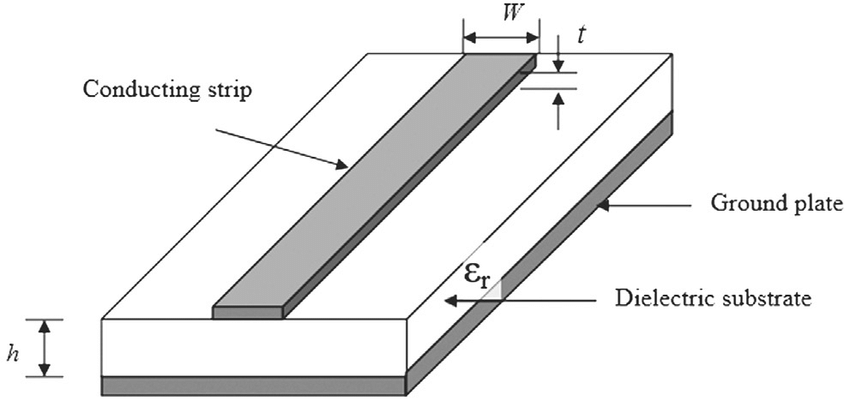
\includegraphics[width=3in]{assets/images/microstrip.png}
    \caption{Microstrip line \cite{microstrip}}
    \label{fig:microstrip}
\end{figure}

Our radio frequency traces are impedance controlled to 50 ohms, which is a standard impedance for radio equipment,
including the \gls{sma} connectors and antennas used by \gls{cuinspace}.

All radio frequency traces on the board are also kept below the critical length for the 433MHz frequency, which
prevents them from acting as an antenna themselves. \Gls{pcb} trace lengths should not exceed 1/12th of the wavelength
in the dielectric. \cite{critical-length}

Our manufacturer's dielectric constant for the prepreg layer we use on our impedance controlled boards is 4.4.
\cite{jlc-pcb-impedance}. Equation \ref{eq:wavelength} is used to calculate the wavelength of the radio signal in the
PCB trace.

\begin{equation}
    \lambda = \frac{c}{f\sqrt{\epsilon_R}}
\end{equation} \label{eq:wavelength}

Then, given this wavelength, the critical length is calculated using Equation \ref{eq:critlen}.

\begin{equation}
    L = \frac{1}{12} \times \lambda
\end{equation} \label{eq:critlen}

The critical length of the trace for our operating frequency of 433.5MHz is approximately 2.75 centimetres. All of our
\gls{rf} traces carrying 433.5MHz signals will therefore be designed to have a total length less than 2.75 centimetres.

\begin{gather*}
    \lambda = \frac{300 \times 10^6}{(433.5 \times 10^6)\sqrt{4.4}} \\
    \lambda = 0.32991785095003 \\
    \\
    L = \frac{1}{12} \times (0.32991785095003) \\
    L = 0.027493154245836 \\
    L \approx 0.0275 \\
\end{gather*}

In addition, our \gls{rf} traces will be designed to have no sharp bends. The RN2483 sample application show traces
that have two bends with a radius of 2.0 millimetres. \cite[Sec. 5.1]{rn2483-datasheet} If a bend is necessary, the
design will adhere to this bend radius.

\section{Real-Time Operating System}

The telemetry transmitter will run a \gls{rtos} called Apache NuttX (referred to as NuttX from here onward). NuttX is
an embedded \gls{rtos} which is designed to have an incredibly small footprint through its many configuration options.
\cite{nuttx-about}. It is \gls{posix} compliant and also adheres to several other standards in the embedded systems
space for APIs that are not governed by \gls{posix}. \cite{nuttx-about} It's completely open source under the Apache
2.0 license and provides a host of existing tools and drivers for file systems, memory devices, analog devices and
digital sensors/peripherals. NuttX has an open community forum for getting support and reporting bugs, which has been
an asset during development. \Gls{cuinspace} is also able to contribute driver code back to the project for the benefit
of others, and has been doing so.

\subsection{Driver Code}

Drivers in NuttX are interacted with via a POSIX interface, composed primarily of the following standard functions:

\begin{itemize}
    \item \texttt{open(const char *path, int oflag, ...)}
    \item \texttt{close(int fildes)}
    \item \texttt{read(int fildes, void *buf, size\_t nbyte)}
    \item \texttt{write(int fildes, void *buf, size\_t nbyte)}
    \item \texttt{ioctl(int fildes, int request, ...)}
\end{itemize}

This allows devices to be interacted with through the regular path name space, just like files. This is standard for
Unix systems, and makes writing application code incredibly convenient.

A major benefit of NuttX's \gls{posix} interface is code portability. By abstracting away low-level code through
drivers which act as files, application code can run on any other \gls{posix} system. This opens up testing
possibilities that allow developers to write and debug application code on their own Linux/MacOS machines before
flashing the microcontroller.

NuttX also supplies drivers of its own for very standard communication protocols such as \gls{uart}, \gls{i2c},
\gls{spi}, etc. This facilitates the writing of device drivers for simple digital sensors such as an \gls{imu} or
temperature sensor.

\subsection{Scheduling}

Task scheduling within NuttX can be easily performed using \gls{posix} \glspl{api} again. It is possible to create
multiple processes or threads which are scheduled by the operating system using a methodology chosen by the developer
(first-in-first-out, round robin, etc.). This also allows \gls{io} operations to be performed alongside the processor
performing application logic.

\Gls{cuinspace} will be leveraging scheduling features to write multi-threaded programs. This allows us to split tasks
by priority and ensure that the highest priority tasks are given time in the processor. In the case of the telemetry
system, highest priority will be given to data logging and radio transmission operations, since those require very
little processor time and only have to trigger short bursts of \gls{io} operations.

\textbf{Task priorities from highest to lowest:}

\begin{enumerate}
    \item Radio transmission
    \item SD card logging
    \item Sensor data collection
\end{enumerate}

Radio transmission is the slowest of the tasks due to radio bandwidth. It will spend most of its time waiting for
\gls{io} operations to complete, so it should have the highest priority. This allows it to perform any \gls{cpu} based
logic quickly and return to blocking, ensuring that the radio operates at its maximum speed.

SD card logging is also \gls{io} intensive, but much quicker in comparison to the radio. It can be prioritized lower
than the radio task for this reason.

Both SD card logging and radio transmission require data to be available to perform their tasks, and will block
otherwise. The sensor data collection thread can therefore run at lowest priority, because whenever the supply of data
is depleted by the radio and logging tasks, it will be given the CPU to produce more data.

The telemetry system will immediately perform boot operations to load all the device drivers before launching into the
application code at power-on.

\section{Data Delivery}

Data logging during flight will be done in a significantly more robust manner than previous years. This involves more
physically secure memory for logging, as well as power-failure guarantees. \Gls{cuinspace} will also be conserving
space through lift-off and landing detection.

Data transmission has worked reliably from a protocol standpoint, and the previous design will be continued and
expanded upon.

\subsection{Data Log Integrity}

The physical memory being used for flight data logging is a standard microSD card. This memory was chosen because it is
cheap, ubiquitous, has an extremely large capacity and is easy to remove for data analysis on a computer immediately
after the rocket is recovered.

One of the challenges posed by an SD card is that it is designed to be removable in nature. SD card slots for quick
removal do not fare well in high vibration and high shock force environments like a rocket. They create a risk for the
SD card to fall out in flight, and also an opportunity for vibrations to temporarily break the electrical connection
between the card and the \gls{mcu}.

To address these risks, \gls{cuinspace} is securing the SD card in a cage-like slot, specifically manufactured to
survive shock loads of up to 50g and have electronic discontinuity for only up to 1 microsecond.
\cite{sd-cage-datasheet} An image of this microSD slot can be seen in \Cref{fig:sd-card-cage}.

\begin{figure}[H]
    \centering
    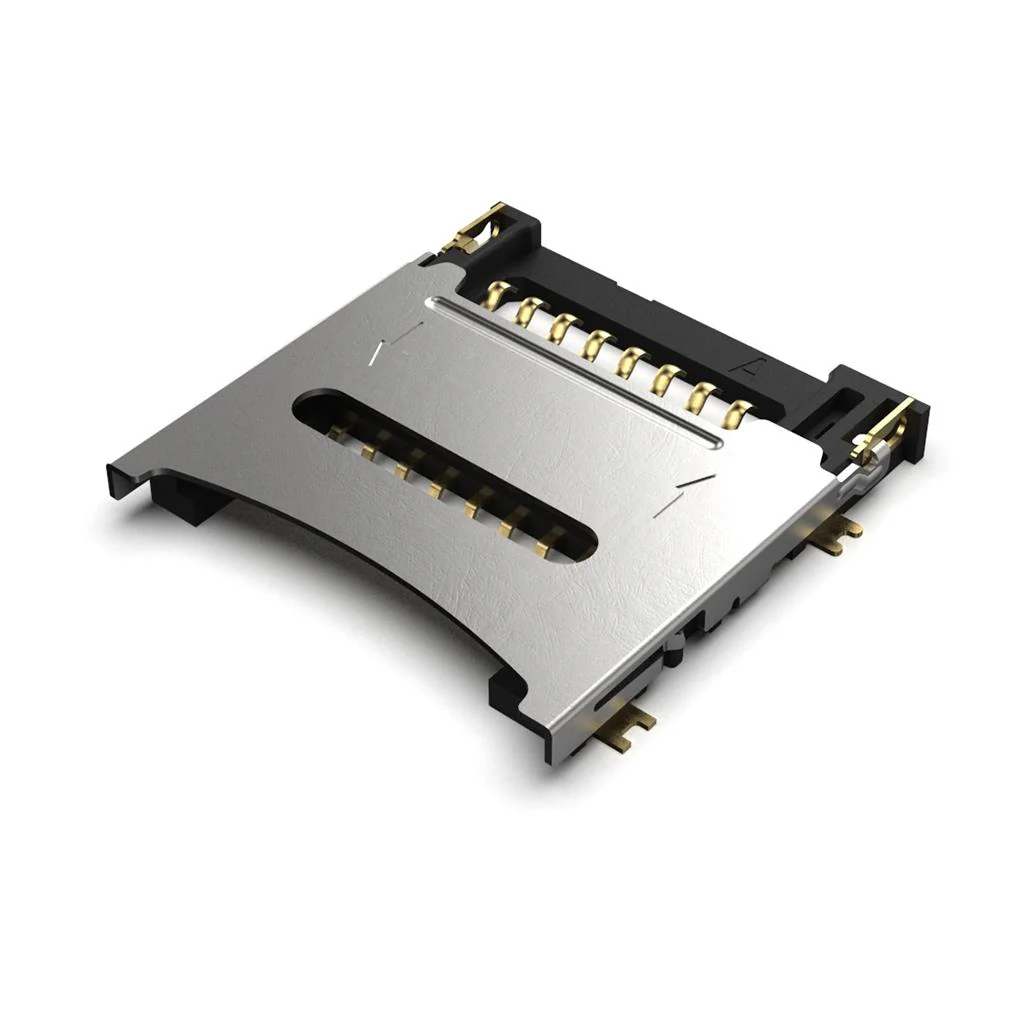
\includegraphics[width=2in]{./assets/images/sd-card-cage.png}
    \caption{Shock load resistant microSD card slot \cite{sd-card-cage}}
    \label{fig:sd-card-cage}
\end{figure}

In order to mitigate discontinuity risks on the software side, the microSD card will make use of the \textit{littlefs}
file system, which provides power-failure safety guarantees. Any brief discontinuity during a write to the SD card will
not corrupt any data, thus preserving the integrity of all logs. You can read more about \textit{littlefs} in
\Cref{apx:littlefs}.

In addition to the \textit{littlefs} file system on the microSD card, there will also be a FAT file system partition.
This partition allows for easy viewing of the telemetry data on a laptop immediately after recovery, as the FAT file
system is accessible through the file explorer on both Windows and Linux computers. Logged flight data is copied from
the \textit{littlefs} partition to the FAT partition upon landing, when there is very little risk of vibrations
corrupting the transfer. The FAT partition will be the first partition on the microSD's partition table so that it is
detected properly on Windows machines.

\subsection{Logging Space Conservation}

In order to preserve logging space and avoid filling up memory with telemetry data being collected while the rocket is
idle on the launch rail, we will be using lift-off and landing detection to trigger logging operations. The \gls{fsm}
used to govern this portion of the system can be seen in \Cref{fig:logging-fsm}.

\begin{figure}[H]
    \centering
    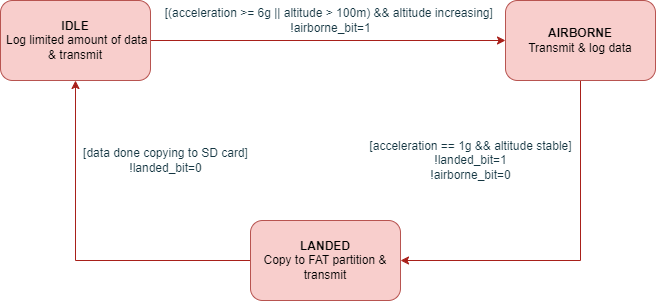
\includegraphics[width=4in]{./assets/diagrams/Flight State FSM.png}
    \caption{Logging control \gls{fsm}}
    \label{fig:logging-fsm}
\end{figure}

Last year, much of the logged telemetry data was captured while the rocket was idle on the launch rail. This is the
\textit{IDLE} state in \Cref{fig:logging-fsm}. In this state we continue to transmit telemetry because it's necessary
to confirm the system's operation and a stable radio signal, but we do not log continuously. Instead, logs are recorded
for only the past 30 seconds at any given time. This gives the system breathing room for latency when detecting
lift-off, without losing any critical data about the start of the launch.

Lift-off is detected using the accelerometer data in conjunction with the barometric pressure sensor. The accelerometer
data can detect the high g-force experienced at launch (previous launches have seen up to 24g) and the barometric
pressure sensor can detect a climbing altitude. In the first few seconds of lift-off, the system will be able to detect
the high g-force and increasing acceleration, at which point it will move to the \textit{AIRBORNE} state. This state is
recorded by setting the "airborne bit" to 1 in the on-board \gls{eeprom}. Doing so means that if the system experience
power-failure in the air, when it reboots it will successfully boot into the \textit{AIRBORNE} state again.

In the \textit{AIRBORNE} state, the flight computer will continuously log to the \textit{littlefs} partition on the SD
card. This will capture flight data at a much higher frequency than is possible to transmit over radio.

Eventually, once the rocket has deployed its chutes at apogee and descended to the ground, the system will detect
landing. The criteria for landing detection is an accelerometer reading of maximum 1g (with slight tolerance for noise)
in any axes combined with a stable altitude which is at ground level. This should prevent landing detection from
triggering while the rocket is at apogee or descending slowly, at which point its altitude will still be quite high and
it should be descending at a larger acceleration than 1g. These thresholds will be configurable and will be set prior
to flight based on simulations on descent speed by the recovery team.

Once the landing is detected, the system will enter the \textit{LANDED} state. In this state the "airborne bit" will be
set to 0 and the "landed bit" will be set to 1. The system will begin copying all logged flight data from the
\textit{littlefs} partition to the FAT file system partition on the SD card. During this time it continues to transmit
telemetry over radio.

Once all the data is copied over, the "landed bit" will be set to 0, and the system will re-enter the \textit{IDLE}
state. At this point, the system still continues transmitting GPS coordinates for recovery, and all flight logs are
safe on the SD card for post-flight extraction. Logs on the \textit{littlefs} partition are only over-written when the
system re-enters the \textit{AIRBORNE} state, which is not possible to trigger from the ground.

\subsection{Data Transmission}

The other method in which \gls{cuinspace} records telemetry data is via live radio broadcasting while the radio is in
flight. This allows a downlink ground station to receive real-time updates about the rocket state while it is in-
flight.

In order to transmit telemetry data over radio, \gls{cuinspace} has developed a radio packet encoding format. This
format can be found in Appendix \ref{apx:comm-spec-repos}. The format covers multiple different data types that are
recorded about the rocket state, such as altitude, acceleration, \gls{gps} coordinates, etc. \cite{radio-comms}.
Importantly, each radio packet starts with a header containing the amateur radio call-sign of the \gls{cuinspace}
operator responsible for flying the system. \cite{radio-comms} The original specification did not include sufficient
space to append a call-zone indicator to the call-sign, which has since been amended in the latest version. This is a
requirement for Canadians broadcasting in the United States \cite{foreign-broadcast}, as \gls{cuinspace} does at
\gls{sac}.

Since \gls{cuinspace}'s rockets achieve altitudes up to around 9 kilometres, it is necessary to choose a radio unit
that can transmit up to such a long range. Unfortunately, long range transmissions are achieved with a trade-off in
bandwidth. This means that the radio unit is not always able to match the measurement speed of the telemetry system.
The on-board data logging is fast enough to capture the full resolution of measured data, but since the radio has low
bandwidth, it is only used to broadcast the most recently measured packet at the time when it becomes ready for another
transmission.

\section{Enclosure Design}

The avionics enclosure is designed to be mounted on top of a bulkhead. In CR25 (the \gls{cots} solid motor rocket), the
enclosure will be mounted inside a fibreglass nosecone for radio transparency. In CR25-H (the hybrid motor), the
enclosure will be mounted inside a fibreglass section of the body tube.

The enclosure shape is still being finalized as aerostructures finishes the bulkhead design.

The enclosure will be stress and shock load tested in simulation to verify structural integrity. It will also be
subjected to vibration testing to ensure that mounting hardware like nuts and screws stay secure.

The enclosure will be made of aluminum to stay lightweight. Most of the weight in the avionics systems mass budget
should be allocated for the batteries.
